\documentclass[a4paper]{article}
\usepackage[margin=0.9in]{geometry}
\usepackage[utf8]{inputenc}
\usepackage{pdfpages}
\usepackage{graphicx}
\usepackage{placeins}

\title{Visualization - Exercise 01}
\author{
    Silas Hoffmann \\
    \texttt{22234721}
    \and
    Katharina Walter \\
    \texttt{21674744}
    \and
    Leonhard Braun \\
    \texttt{21679325}
}
\date{\today}


\begin{document}

    \maketitle


    \section{Exercise 1.1: applying Tufte's design principles}

    \subsection{Discussion - \textit{baseball.png}}

    \subsubsection{Tuffte - Elements that are not \textbf{data ink}}
    \begin{itemize}
        \item Arrows in the label
        \item Time-axis
        \item Team Logos
        \item the colors in general since the do not add any meaning
    \end{itemize}

    \subsubsection{Dos and Dont's}
    \begin{itemize}
        \item \textbf{show full y-axis:} not present
        \item \textbf{consistent x-axis intervals}: not present
        \item \textbf{Edward Tufte in a nutshell - remove clutter}: is full of clutter, not very neatly organized
        \item \textbf{highlight what’s important}: in essence the main points are highlighted, but it can be conveyed much simpler
        \item \textbf{sorting}: Data is sorted
        \item \textbf{do not use 3d or other visual effects}: no 3d effects
        \item \textbf{direct labeling where possible}: done correctly
        \item \textbf{avoid pie charts}: done correctly - isn't a pie chart
        \item \textbf{avoid stacked charts}: done correctly - isn't a stacked chart
        \item \textbf{do not use maps for everything with spatial dimension}: done correctly
        \item \textbf{avoid animations, use small multiples}: done correctly - isn't an animation
        \item \textbf{show level of confidence}: accurate, although not explicitly given
        \item \textbf{tell the ‘why’ and ‘how’}: not implemented, hard to understand
        \item \textbf{how to treat missing data}: not indicated
        \item \textbf{do not confuse causation and correlation}: not present
        \item \textbf{do not compare apples with oranges}: at first glance it is unclear what the data should display,
        but if the underlying article examines the displayed coherence it can be correctly used
        \item \textbf{adjust for inflation}: all data points come from the same year - no adjustment necessary
        \item \textbf{do not forget color deficiency}: no information is bound to a color
    \end{itemize}

    The following figure displays how we would implement the principles from the lecture.
    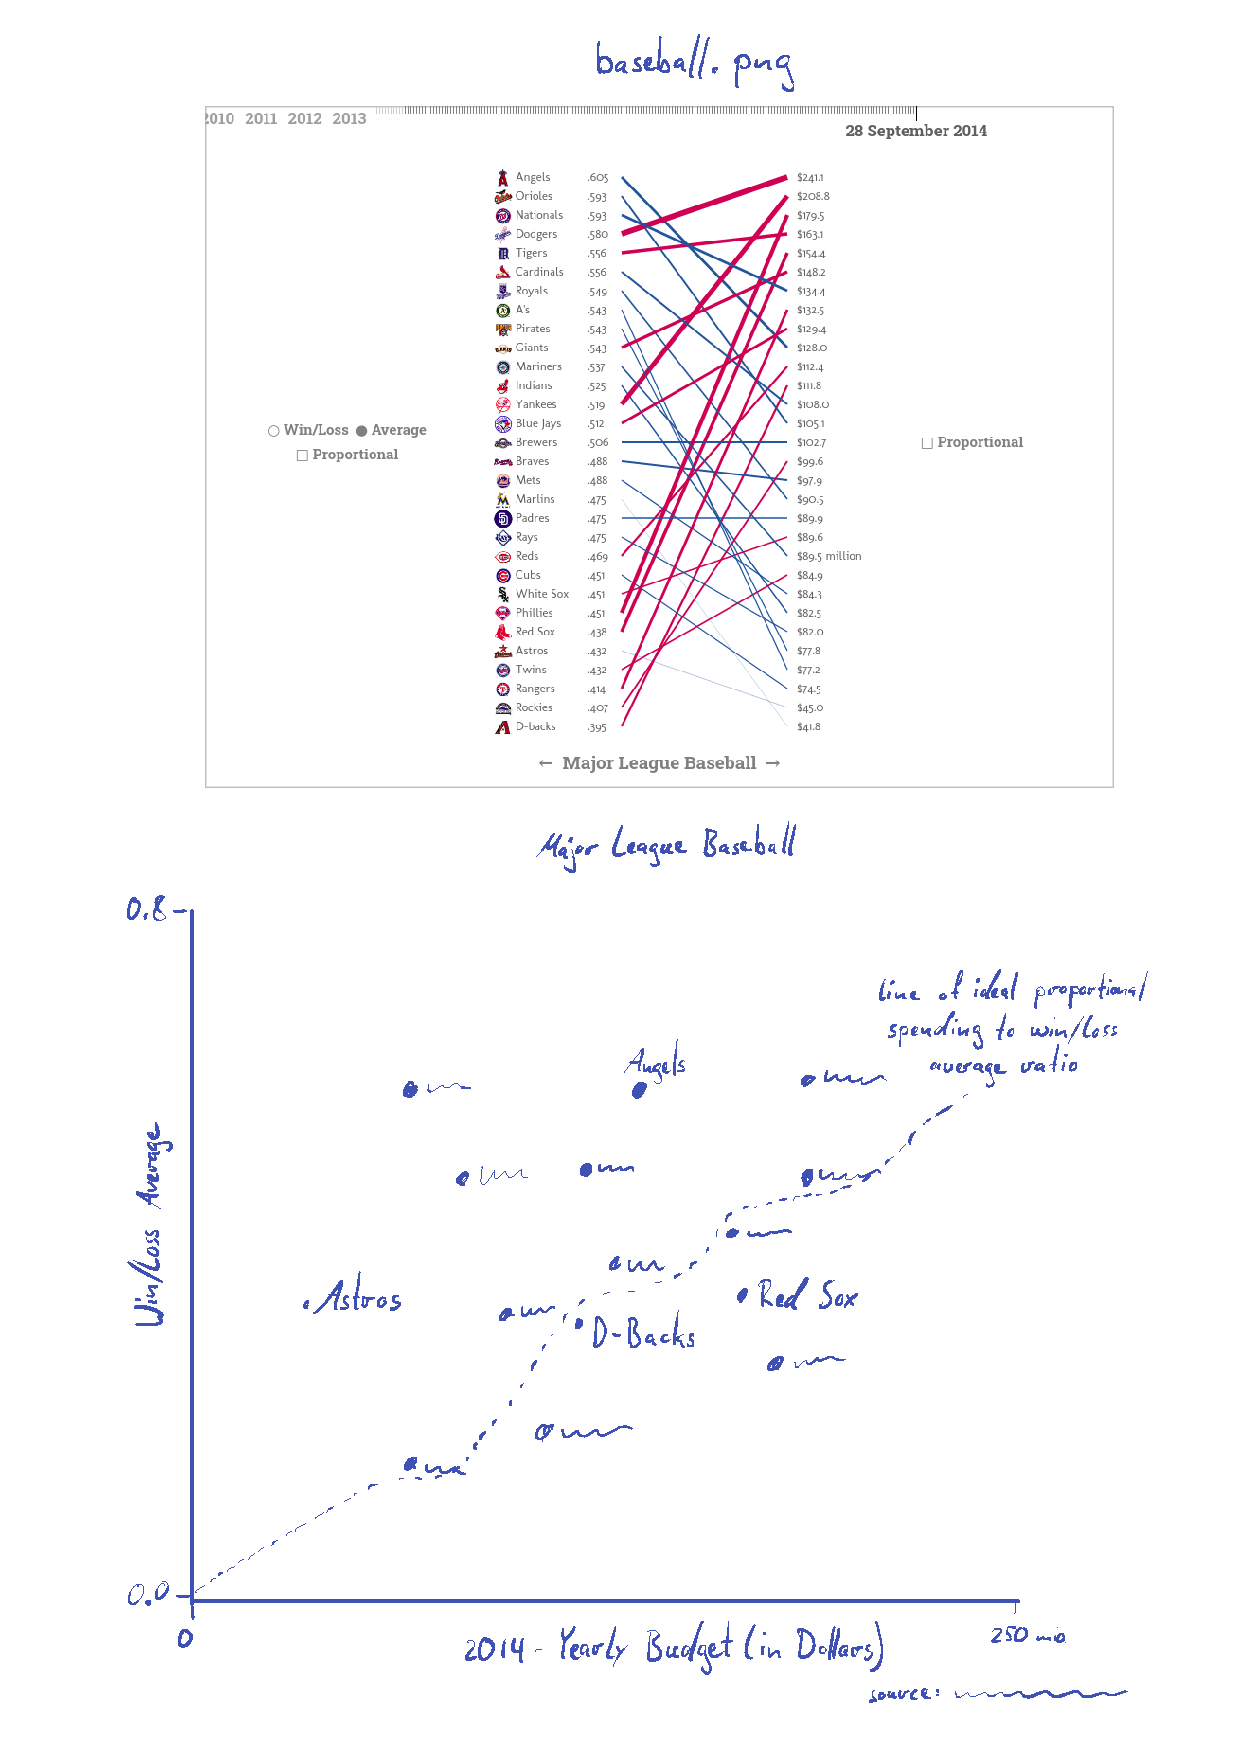
\includepdf[pages=1]{./attachments/vis-01_ex01_img.pdf}


    \subsection{Discussion - \textit{energy.png}}

    \subsubsection{Tuffte - Elements that are not \textbf{data ink}}
    \begin{itemize}
        \item The logos displaying the different sectors
        \item 3d Animation
    \end{itemize}

    \subsubsection{Dos and Dont's}
    \begin{itemize}
        \item \textbf{show full y-axis:} implemented correctly, although maybe it would be better to ramp up the y-axis to 100 \%
        \item \textbf{consistent x-axis intervals}: present and consistent
        \item \textbf{Edward Tufte in a nutshell - remove clutter}: the chart actually displays two separate graphs in one
        \item \textbf{highlight what’s important}: done correctly
        \item \textbf{sorting}: Data is sorted
        \item \textbf{do not use 3d or other visual effects}: 3d effects present - could be improved
        \item \textbf{direct labeling where possible}: done partially through the images - could be done better (with text)
        \item \textbf{avoid pie charts}: done correctly - isn't a pie chart
        \item \textbf{avoid stacked charts}: done correctly - isn't a stacked chart
        \item \textbf{do not use maps for everything with spatial dimension}: done correctly
        \item \textbf{avoid animations, use small multiples}: done correctly - isn't an animation
        \item \textbf{show level of confidence}: accurate, although not explicitly given
        \item \textbf{tell the ‘why’ and ‘how’}: since the sources is cited, this could be interpreted as the ‘how’
        but the ‘why’ is missing
        \item \textbf{how to treat missing data}: not indicated
        \item \textbf{do not confuse causation and correlation}: not present
        \item \textbf{do not compare apples with oranges}: all data-points seem compatible
        \item \textbf{adjust for inflation}: not necessary since the data does not display monetary value
        \item \textbf{do not forget color deficiency}: no information is bound to a color.
        So, although color is used in the chart, a colorblind person still can convey the meaning of the graph without any problems.
    \end{itemize}

    The following figure displays how we would implement the principles from the lecture.
    \includepdf[pages=2]{./attachments/vis-01_ex01_img.pdf}


    \subsection{Discussion - \textit{machine-learning.png}}

    \subsubsection{Tuffte - Elements that are not \textbf{data ink}}
    \begin{itemize}
        \item pattern in the posts seem unnecessary distracting
    \end{itemize}

    \subsubsection{Dos and Dont's}
    \begin{itemize}
        \item \textbf{show full y-axis:} is present, but no measurement unit provided
        \item \textbf{consistent x-axis intervals}: present and consistent
        \item \textbf{Edward Tufte in a nutshell - remove clutter}: seems ok, but the pattern in the post make the
        whole chart confusing
        \item \textbf{highlight what’s important}: done correctly
        \item \textbf{sorting}: Data is sorted
        \item \textbf{do not use 3d or other visual effects}: 3d effects present - could be improved
        \item \textbf{direct labeling where possible}: implemented through a legend - could be improved
        \item \textbf{avoid pie charts}: done correctly - isn't a pie chart
        \item \textbf{avoid stacked charts}: done correctly - isn't a stacked chart
        \item \textbf{do not use maps for everything with spatial dimension}: done correctly
        \item \textbf{avoid animations, use small multiples}: done correctly - isn't an animation
        \item \textbf{show level of confidence}: not present
        \item \textbf{tell the ‘why’ and ‘how’}: not present - no source, no further information, no heading,
        legend without context highly confusing
        \item \textbf{how to treat missing data}: not indicated
        \item \textbf{do not confuse causation and correlation}: not present
        \item \textbf{do not compare apples with oranges}: due to lack of context not able to draw conclusion
        \item \textbf{adjust for inflation}: not necessary since the data does not display monetary value
        \item \textbf{do not forget color deficiency}: done correctly
    \end{itemize}

    The following figure displays how we would implement the principles from the lecture.
    \includepdf[pages=3]{./attachments/vis-01_ex01_img.pdf}

    \clearpage

    \section{Exercise 1.2: a first visualization task.}
    \FloatBarrier
    \begin{figure*}[!ht]
        \centering
        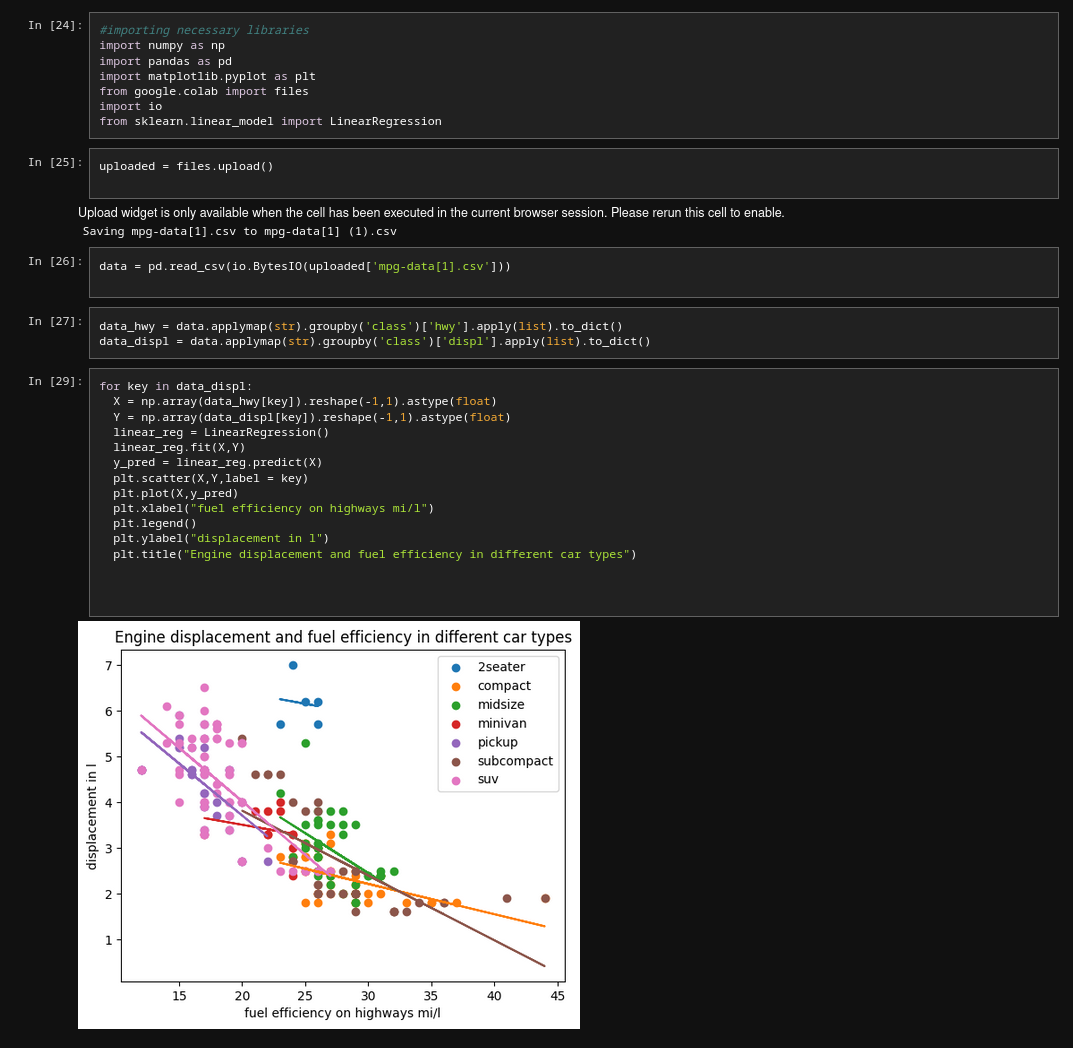
\includegraphics[width=\textwidth,height=\textheight,keepaspectratio]{./attachments/VisZettel1-export}
        \caption{Screenshot from Jupyter Notebook}
    \end{figure*}

\end{document}
